\documentclass[a4paper]{article} 
\input{head}
\begin{document}

%-------------------------------
%	TITLE SECTION
%-------------------------------

\fancyhead[C]{}
\hrule \medskip % Upper rule
\begin{minipage}{0.295\textwidth} 
\raggedright
\footnotesize
Büşra Bahadir \hfill\\   

\end{minipage}
\begin{minipage}{0.4\textwidth} 
\centering 
\large 
ÖDEV 1\\ 
\normalsize 
EMEK EKONOMİSİ-İKT 533\\ 
\end{minipage}
\begin{minipage}{0.295\textwidth} 
\raggedleft
\today\hfill\\
\end{minipage}
\medskip\hrule 
\bigskip

%-------------------------------
%	CONTENTS
%-------------------------------


a) 3 adet doğum çeğreği kukla değişkeni oluşturuyoruz.Eğitimin ücretler üzerindeki etkisi analiz edilirken doğum çeyrekleri eğitim için enstrüman değişken olarak kullanılır. Dolayısyla doğum çeyrekleri enstrüman değişken iken enstrüman değişkenin eğitim üzerindeki etkisini test eden regresyon birinci aşama (first stage) olacaktır. Bu tahminin katsayısı 0 olmaz.Yani enstrüman biraz açıklayıcı güce sahiptir. İndirgenmiş form (reduced form) ise ücretler ve enstrüman değişken doğum çeyrekleri arasındaki ilişkiyi tahminleyen modeldir.
\item
Birinci aşama tahminleri Tablo 3 deki Panel A ve Panel B deki ikinci sütundaki 3. kolondaki doğum ceyreğinin eğitim üzerindeki etkisini inceleyen tahmindir. [-0.1256(0.0155) ve -0.1088(0.0132)].
İndirgenmiş form tahminleri ise enstrüman değişken doğum çeyreğinin ücretler üzerindeki regresyonundan bulduğumuz Panel A ve Panel B ' deki ilk sütundaki 3.kolondaki tahminlerdir. [-0.00898(0.00301) ve -0.01110(0.00274)]. İndirgenmiş form katsayılarını alıp birinci aşama katsayılarına bölersek Wald tahminlerini elde ederiz. Wald tahmini, ilk çeyrekle diğer 3 çeyrek arasındaki ĕgitimdeki genel farkla tanımlanır
.
\item
\item
\item
\begin{table}[h!]
\centering 
\begin{tabular}{@{}lccc@{}}
\toprule
\multicolumn{4}{l}{PANEL A: WALD ESTIMATES FOR 1970 CENSUS - MEN BORN 1920-1929}                                                                                                                                                                                                                      \\ \midrule
                                 & \begin{tabular}[c]{@{}c@{}}(1)\\ Born in \\ 1st quarter \\ of year\end{tabular} & \begin{tabular}[c]{@{}c@{}}(2)\\ Born in 2nd, \\ 3rd, or 4th\\  quarter of year\end{tabular} & \begin{tabular}[c]{@{}c@{}}(3)\\ Difference\\ (std. error)\\ (1)-(2)\end{tabular} \\ \midrule
ln (wkly. wage)                  & 5.1484                                                                        & 5.1574                                                                                      & \begin{tabular}[c]{@{}c@{}}-.00898\\ (.00301)\end{tabular}                    \\
Education                       & 11.3996                                                                         & 11.5252                                                                                     & \begin{tabular}[c]{@{}c@{}}-.1256\\ (.0155)\end{tabular}                    \\
Wald est. of return to education &                                                                                 &                                                                                              & \begin{tabular}[c]{@{}c@{}}.0715\\ (.0219)\end{tabular}                     \\
OLS return to education         &                                                                                 &                                                                                              & \begin{tabular}[c]{@{}c@{}}.0801\\ (.0004)\end{tabular}                     \\ \midrule
\multicolumn{4}{l}{PANEL B: WALD ESTIMATES FOR 1980 CENSUS - MEN BORN 1930-1939}                                                                                                                                                                                                                      \\ \midrule
                                 & \begin{tabular}[c]{@{}c@{}}(1)\\ Born in \\ 1st quarter \\ of year\end{tabular} & \begin{tabular}[c]{@{}c@{}}(2)\\ Born in 2nd,\\  3rd, or 4th \\ quarter of year\end{tabular} & \begin{tabular}[c]{@{}c@{}}(3)\\ Difference\\ (std. error)\\ (1)-(2)\end{tabular} \\ \midrule
ln (wkly. wage)                 & 5.8916                                                                        & 5.9027                                                                                     & \begin{tabular}[c]{@{}c@{}}-.01110\\ (.00274)\end{tabular}                    \\
Education                       & 12.6881                                                                        & 12.7969                                                                                     & \begin{tabular}[c]{@{}c@{}}-.1088\\ (.0132)\end{tabular}                    \\
Wald est. of return to education &                                                                                 &                                                                                              & \begin{tabular}[c]{@{}c@{}}.1020\\ (.0239\end{tabular}                      \\
OLS return to education          &                                                                                 &                                                                                              & \begin{tabular}[c]{@{}c@{}}.0709\\ (.0003)\end{tabular}                      \\ \bottomrule
\end{tabular}

\end{table}
\\
\\
\\
\\
\\
\\
\\
\\
\\

\newpage 
b) Wald tahmini enstrüman değişkenin özel bir durumu gibidir.
Bu durumda Wald tahmini, bir bireyin yılın ilk çeyreğinde doğup doğmadığını gösteren bir kukla değişkenin eğitim için bir araç olarak kullanıldığı ve hiçbir kontrol değişkeninin bulunmadığı araç değişkenlere eşdeğerdir. TSLS tahminleri iki önemli açıdan Wald tahminlerinden farklılık gösterir. İlk olarak, TSLS tahminleri kontrol değişkenleri içerir. İkincisi, TSLS modelleri, her yıl doğumun her çeyreğindeki eğitimdeki varyasyonlarla tanımlanırken, Wald tahmini, ilk çeyrek ile yılın geri kalanı arasındaki eğitimdeki genel farkla tanımlanır.
\item
\item
Aşağıdaki tablolar her iki dönem (1920-29 ve 1930-39) için aynı araç değişken kullanarak yapılmış, herhangi bir kontrol değişkeni kullanılmayan 2SLS tahminlerini (Wald Tahmini), bütün ırk, bölge kuklaları, doğum yılı kuklaları ve yaş değişkeni kullanılarak yapılmış 2SLS tahminlerini, herhangi bir kontrol değişkeni kullanılmadan yapılmış OLS tahminlerini ve bütün kontrol değişkenlerin birlikte kullanıldığı OLS tahminlerini içermektedir.
Eğitim yılı için doğum çeyrekleri enstrüman değişken olarak kullanılmıştır. her iki dönem için birinci dönem için 1970, ikinci dönem için 1980 nüfus sayımı verileri kullanılarak aynı tahminler yapılmış ve aşağıdaki iki tabloda ayrı ayrı sunulmuştur. Tablolardaki birinci sütun ve üçüncü sütunlar OLS tahminlerini, ikinci ve dördüncü sütunlar 2SLS tahminlerini göstermektedir. 
\item
İlk tablo 1970 nüfus sayımı verileri kullanılarak yapılmış 1920-29 dönemine ait tahminleri içermektedir. Tabloya bakıldığında herhangi bir kontrol değişkeni kullanılmadan yapılmış OLS ve 2SLS tahminlerinin (1. ve 2. sütun) a şıkkında oluşturulan OLS ve Wald tahminleri ile aynı olduğu görülecektir. Kontrol değişkenleri eklenerek yapılmıs OLS ve 2SLS tahminlerinde ise yaş dışında bütün açıklayıcı değişkenler istatistiki olarak anlamlı bulunmuştur. OLS tahmininde kontrol değişkenleri eklendiğinde eğitimin katsayısı düşerken 2SLS taminlerinde bu katsayı artmıştır. Doğum yılı kuklaları ücret eşitliklerine dahil edildiğinden,  eğitimin etkisi her doğum yılı içinde doğum çeyrekleri arasındaki eğitimdeki farklılıkler (varyasyon) olarak tanımlanır. Bu yüzden 3. ve 4. sütunlar ilk 2 sütunu tekrar ederler doğum yılı kuklalarını da dahil ederler. Bunlara ek olarak diğer bütün kontrol değişkenleri de kullanılmıştır. 

\item


\begin{table}[htbp]\centering
\def\sym#1{\ifmmode^{#1}\else\(^{#1}\)\fi}

\begin{tabular}{l*{4}{c}}
\hline\hline
Independent Variables   &\multicolumn{1}{c}{\begin{tabular}[c]{@{}l@{}}(1)\\ OLS\end{tabular}}&\multicolumn{1}{c}{\begin{tabular}[c]{@{}l@{}}(2)\\  TSLS)\end{tabular}}&\multicolumn{1}{c}{\begin{tabular}[c]{@{}l@{}}(3)\\ OLS\end{tabular}}&\multicolumn{1}{c}{\begin{tabular}[c]{@{}l@{}}(4)\\ TSLS\end{tabular}}\\
\hline
Years of education       &      0.0802\sym{***}&      0.0715\sym{***}&              0.0701\sym{***}&       0.1007\sym{**} \\
                         &  (0.0004)         &    (0.0219)              &  (0.0004)         &    (0.0334)         \\
[1em]
Race(1 = black)          &                     &                     &                       -0.298\sym{***}&      -0.227\sym{**} \\
                         &                     &                     &                             (0.0043)         &    (0.0776)         \\
[1em]
SMSA (1 = center city)   &                     &                     &                      -0.134\sym{***}&      -0.116\sym{***}\\
                         &                     &                     &                      (0.0026)         &    (0.0198)         \\
[1em]
Married (1 = married)    &                     &                     &                                     0.293\sym{***}&       0.280\sym{***}\\
                         &                     &                     &                        (0.0037)         &    (0.0141)         \\
8 Region of residence dummies     &          No           &       No              &                                               Yes&       Yes\\
                         &                     &                     &                                   &           \\                       
[1em]
9 Region of residence dummies     &          No           &      No               &                                               Yes&       Yes\\
                         &                     &                     &                                    &          \\   
[1em]
Age                      &                     &                     &                       0.116         &       0.117         \\
                         &                     &                     &                (0.0652)         &    (0.0661)         \\
[1em]
Age-squared              &                     &                     &        -0.00125         &    -0.00118         \\
                         &                     &                     &            (0.0007)         &  (0.0007)         \\
\hline
Observations             &      247199         &      247199         &      247199       &  247199         \\
\hline\hline
\multicolumn{9}{l}{\footnotesize Standard errors in parentheses}\\
\multicolumn{9}{l}{\footnotesize \sym{*} \(p<0.05\), \sym{**} \(p<0.01\), \sym{***} \(p<0.001\)}\\
\end{tabular}
\end{table}
\end{landscape}
\clearpage
İkinci tablo ise 1980 nüfus sayımı verileri kullanılarak yapılmış 1930-39 dönemine ait tahminleri içermektedir. Birinci tabloda yapılmış olan tahminlerin aynısı bu tabloda yapılmıştır. Bu dönemde kontrol değişkenleri eklendiğinde OLS ve TSLS tahminlerine ait eğitim değişkenine ait katsayıların (3. ve 4. sütunda) azaldığı görülmektedir. Bu tabloda da önceki tablo ile aynı şekilde yaş dışındaki bütün kontrol değişkenleri istatistiki olarak anlamlıdır.

\begin{landscape}
\begin{table}[htbp]\centering
\def\sym#1{\ifmmode^{#1}\else\(^{#1}\)\fi}

\begin{tabular}{l*{4}{c}}
\hline\hline
Independent Variables   &\multicolumn{1}{c}{\begin{tabular}[c]{@{}l@{}}(1)\\ OLS\end{tabular}}&\multicolumn{1}{c}{\begin{tabular}[c]{@{}l@{}}(2)\\ TSLS\end{tabular}}&\multicolumn{1}{c}{\begin{tabular}[c]{@{}l@{}}(3)\\ OLS\end{tabular}}&\multicolumn{1}{c}{\begin{tabular}[c]{@{}l@{}}(4)\\  TSLS\end{tabular}}\\
\hline
Years of education       &      0.0709\sym{***}&      0.1020\sym{***}&            0.0632\sym{***}&      0.0600\sym{*}  \\
                         &  (0.0003)         &    (0.0239)                 &  (0.0003)         &    (0.0290)         \\
[1em]
Race(1 = black)          &                     &                     &                           -0.257\sym{***}&      -0.263\sym{***}\\
                         &                     &                     &                         (0.0040)         &    (0.0458)         \\
[1em]
SMSA (1 = center city)   &                     &                     &                          -0.176\sym{***}&      -0.180\sym{***}\\
                         &                     &                     &                                (0.0029)         &    (0.0305)         \\
[1em]
Married (1 = married)    &                     &                     &                                               0.248\sym{***}&       0.249\sym{***}\\
                         &                     &                     &                            (0.0032)         &   (0.0073)         \\
[1em]
8 Region of residence dummies     &          No           &       No              &                                               Yes&       Yes\\
                         &                     &                     &                                   &           \\                       
[1em]
9 Region of residence dummies     &          No           &      No               &                                               Yes&       Yes\\
                         &                     &                     &                                    &          \\   
Age                      &                     &                     &          -0.0760         &     -0.0741         \\
                                 &                     &                     &    (0.0604)         &    (0.0626)         \\
[1em]
Age-squared              &                     &                     &                           0.0008         &    0.0007         \\
                                &                     &                     &  (0.0007)         &  (0.0007)         \\
\hline
Observations             &      329509         &      329509         &      329509         &      329509         &               \\
\hline\hline
\multicolumn{9}{l}{\footnotesize Standard errors in parentheses}\\
\multicolumn{9}{l}{\footnotesize \sym{*} \(p<0.05\), \sym{**} \(p<0.01\), \sym{***} \(p<0.001\)}\\
\end{tabular}
\end{table}
\end{landscape}
\item
\item
\item

c) Zayıf bir enstrüman değişken , enstrümanı olarak kullanıldığı değişkenle yüksek düzeyde ilişkili olmayan bir enstrümandır, bu nedenle bu enstrümanla ilişkili ilk aşama katsayısı küçüktür veya kesin olarak tahmin edilmez.Bu gibi birçok araç değişkenle yapılan 2SLS tahminleri, aynı modelin OLS tahminlerine benzer olma eğilimindedir. 2SLS, OLS'ye yakın olduğunda, ikincisindeki seçilim yanlılığı konusunda endişelenmenize gerek olmadığı sonucuna varmanız doğaldır, ancak bu sonuç yersiz olabilir. Sonlu örneklem sapması (finite sample bias) nedeniyle, birçok zayıf IV kullanılarak yapılan  2SLS tahminleri, ilginin nedensel ilişkisi hakkında size çok az şey söyler.
\item
Sonlu örneklem sapması ne zaman endişelenmeye değer? Birçok enstrümanla kurulan bütün ilk aşama tahminlerinin sıfır olduğu ortak hipotezini test eden ilk aşama F istatistiğine odaklanılır. Popüler bir genel kurala göre, bunu ortadan kaldırmak için F değerinin en az 10 olması gerekmektedir.  2SLS'ye bir alternatif olarak LIML modeli sonlu örneklem sapmasından daha az etkilenmektedir. Eğer tek bir nedensel etkiyi tahmin etmek için tek bir enstrüman kullanılırsa birçok zayıf araç değişken problemi azaltilabilir.İndirgenmiş form tahminleri sınırlı örneklem sapmasından etkilenmeyen OLS tahminleri olduğundan dikkatle incelenmesi gerekmektedir. Küçük ve anlamlı ölçüde sıfırdan farklı olmayan indirgenmiş form tahminleri en azından eldeki verilerde, ilgili nedensel ilişkinin zayıf veya var olmadığına dair güçlü ve tarafsız bir ipucu sağlar. Çoklu indirgenmiş form katsayıları ayrıca bir F testi kullanılarak birlikte test edilmelidir.
\item
Aşağıdaki tabloda ilk iki sütun B şıkkında 1920-29 için yapılan IV tahminlerinin birinci aşama F istatistiklerini göstermektedir. 3. ve 4. sütunda 1930-39 dönemine ait IV tahminlerinin F istatistikleri mevcuttur. Burada bütün kontrol değişkenleri eklenerek yapılan IV tahminlerinin birinci aşama F istatistiklerinin daha düşük olduğunu 2. ve 4. sütundan görebiliriz. Aynı şekilde bu tahminlerde standard hataların daha düşük olduğunu da görüyoruz.
Doğum çeyreği kukla değişken IV konusuna, ek enstrümanlar ve kontrol değişkenleri eklemek için 2SLS' i  kullanabiliriz.
\item
 \item
 \item
                      \\
     
 \\ \\
 \item


\item

\item
\item
\\

\begin{table}
\def\sym#1{\ifmmode^{#1}\else\(^{#1}\)\fi}
\begin{tabular}{l*{5}{c}}
\hline\hline
   &\multicolumn{1}{c}{\begin{tabular}[c]{@{}l@{}}(1920-1929)\\
         TSLS\end{tabular}}&\multicolumn{1}{c}{\begin{tabular}[c]{@{}l@{}}(1920-1929)\\ TSLS\end{tabular}}&\multicolumn{1}{c}{\begin{tabular}[c]{@{}l@{}}(1930-1939)\\ TSLS\end{tabular}}&\multicolumn{1}{c}{\begin{tabular}[c]{@{}l@{}}(1930-1939)\\  TSLS\end{tabular}}\\
\hline

\item
Years of education       &      .102\sym{}&      .067\sym{}&      .071\sym{}&      .0805\sym{} &                 &       \\
                                &    (.0219)         &  (.0152)         &    (.0240)         &  (.0164)          &                \\
       \\
[1em]
First-stage F-statistic   &        65             &   57,2                  &        67             &                58    &      &     
                         &                     &                     &                     &                     &           \\
[1em]
Instruments    &       Quarter 1              &     Quarter 1                & Quarter 1                     &   Quarter 1                  &          
                         &                     &                     &                     &                     &           \\
[1em]
                \\
[1em]
All control variables              &   No                  &   Yes                  &    No         &    Yes         &                     &                     &           \\
                         &                     &                     &       &                     &                            \\
\hline
\multicolumn{9}{l}{}\\
\multicolumn{9}{l}{\footnotesize }
\end{tabular}
\end{table}
 \item
  Peki bu doğum çeyreği enstrümanları birinci aşama, bağımsızlık ve dışlanmış kısıtlılık gerekliliklerini nasıl hesaplar? Bu tabloda sunulan büyük F istatistikleri güçlü bir ilk aşamanın göstergeleridir. 
 Büyük bir birinci aşama F istatistiği, zayıf araçlardan kaynaklanan yanlılığın bu bağlamda bir sorun olma ihtimalinin düşük olduğunu göstermektedir. Yukarıda da bahsettiğim üzere eğer F istatistiği 10 dan büyükse zayıf araç değişkenden söz edemeyiz. Araç değişkenin güçlü olduğu sonucuna varırız.
 \item
 \clearpage
 d)1930-39 dönemi için yatay eksende doğum çeyreklerinin ve yılların, dikey eksende ise o çeyrekte doğanların eğitim seviyelerinin ortalamalarının yer aldığı çigi grafik aşağıda sunulmuştur.
 
 \begin{figure}[ht!]
\centering

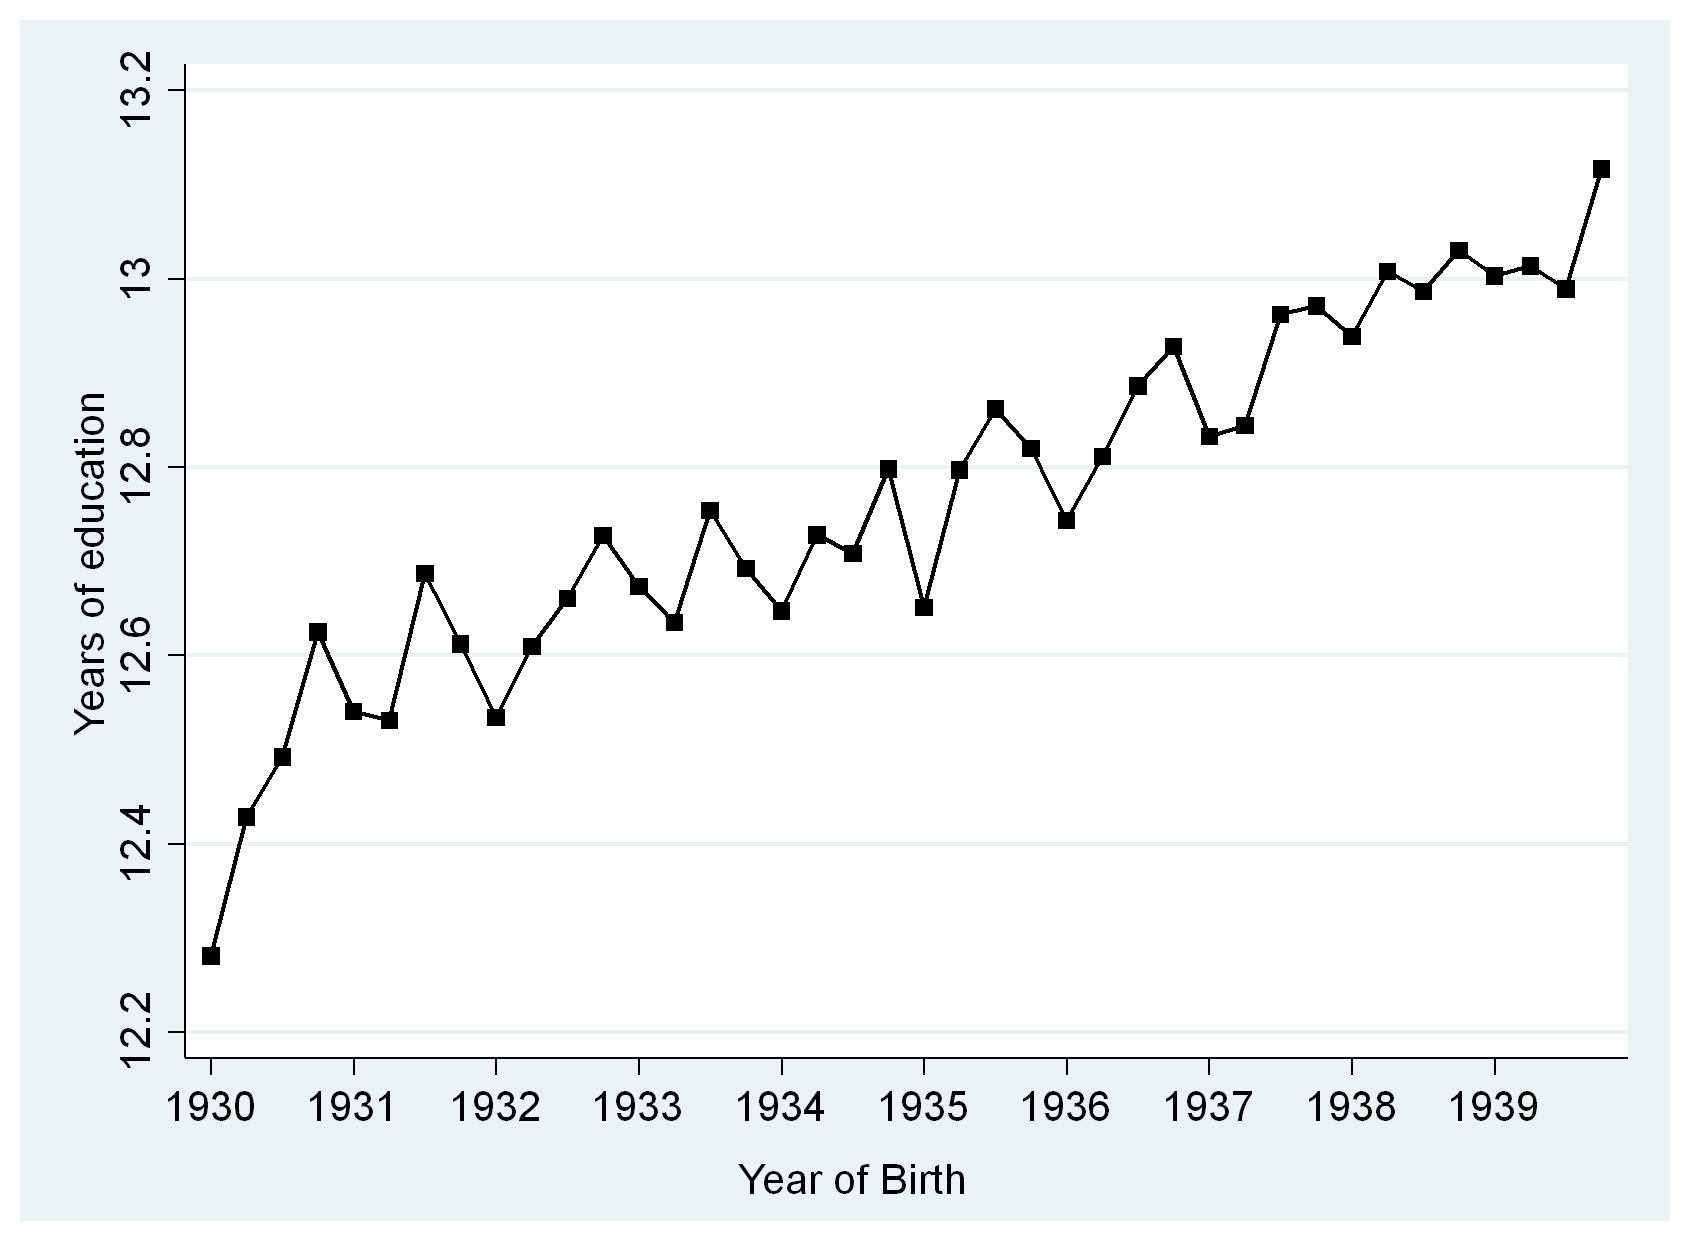
\includegraphics[width=150mm]{busraa.png}
\label{overflow}
\end{figure}
\end{document}
\bigskip
\

%------------------------------------------------

\bigskip

%------------------------------------------------

\end{document}
